\documentclass[12pt]{article}

\usepackage{sbc-template}
\usepackage{textcomp}
\usepackage{listings}
\usepackage{graphicx,url}
\usepackage{framed}
\usepackage{color}
\usepackage[utf8]{inputenc}
\usepackage{fontenc}

% Definição do template de formatação e synthax hightlight para groovy :)
%
\lstdefinelanguage{Groovy}{keywords={
                                            abstract, default, if, private, this,
                                            boolean, do, implements, protected, 
                                            throw, break, double, import, public, 
                                            throws, byte, else, instanceof, return,
                                            transient, case, extends, int, short, 
                                            try, catch, final, interface, static, 
                                            void, char, finally, long, strictfp,
                                            volatile, class, float, native, super, 
                                            while, const, for, new, switch, continue,
                                            goto, package, synchronized, def, any, 
                                            as, in, with, null, true, false, static
                                },
                                keywords={[2]params, render,it, flash, redirect},
                                morecomment=[l]{//},
                                morecomment=[s]{/*}{*/},
                                morestring=[b]",
                                morestring=[d]',
                                morestring=[b]""",
                                morestring=[b]''',
                                morestring=[b]/
                           }

%
%   Definição de estilos das linguagens
%
%\lstdefinestyle{Listagem}{
%                        \lstlistingname
%                        }
\lstdefinestyle{Groovy}{
                            upquote=true,
                            basicstyle=\small,
                            keywordstyle=\color[RGB]{151,40,120},
                            keywordstyle={[2]\color[RGB]{102, 204, 255}},
                            stringstyle={\color[RGB]{255,0,204}
                                         \ttfamily
                                         \small
                            },
                            identifierstyle=\ttfamily,
                            breaklines=true,
                            showtabs=false,
                            showspaces=false,
                            showstringspaces=false,
                            columns=fullflexible,
                            numbers=left,
                            language=Groovy,
                            name=Listagem
                            extendedchars=true,
                            frame=leftline
                       }
\lstdefinestyle{InlineGroovy}{
                           style=Groovy,
                           numbers=none
                      }
\lstdefinestyle{Java}{
                        keywordstyle={\color[RGB]{127,0,85} \ttfamily \small },
                        stringstyle={\color[RGB]{42,0,255} \ttfamily \small},
                        commentstyle={\color[RGB]{63,127,95} \ttfamily \small},
                        upquote=true,
                        basicstyle=\small,
                        breaklines=true,
                        showtabs=false,
                        showspaces=false,
                        showstringspaces=false,
                        columns=fullflexible,
                        numbers=left,
                        language=Java,
                        name=Listagem,
                        frame=leftline                   
                     }

\sloppy

\title{Groovy on Rails, uma alternativa para o desenvolvimento de aplicações web
       sem sair da Plataforma Java}

\author{Marcelo Emanoel Bezerra Diniz\inst{1}}

\address{
    Centro de Ciências Tecnológicas -- Universidade de Fortaleza (UNIFOR)\\
    CEP 60.811-905 -- Fortaleza -- CE -- Brasil
}

\begin{document} 

\maketitle

\begin{resumo} 
    
    Desde seu surgimento a plataforma Java se destaca como uma ótima alternativa
    para o desenvolvimento de aplicações web. Diversos frameworks surgiram para 
    proporcionar reutilização de código e aumento de produtividade. A plataforma
    possui implementações robustas e amplamente utilizadas. Porém, apesar dos 
    esforços, outras tecnologias mais recentes vem se destacando e tomando a 
    frente no cenário de desenvolvimento de aplicações para a web. Dentre estas 
    tecnologias são notórias algumas características como o uso de linguagens 
    dinâmicas em conjunto com padrões de projeto amplamente conhecidos. Neste 
    artigo será abordado o framework Groovy on Rails, ou simplesmente, Grails. 
    O framework alia a linguagem dinâmica groovy
    à arquitetura utilizada no Ruby on Rails. \nocite{*}
    
\end{resumo}

\section{Introdução}

    Alta competitividade, baixo custo de produção e manutenção, além de alta 
    qualidade são exigências do mercado de desenvolvimento de software. 
    Independentemente da tecnologia envolvida no processo de construção de uma 
    aplicação web, existe o componente de complexidade inerente ao próprio 
    ambiente. Toda a comunicação é baseada no protocolo HTTP. Sua simplicidade 
    garante a alta disponibilidade da Web, porém requer um trabalho adicional 
    das aplicações para manter as informações seguras e íntegras.

    No cenário previamente descrito, a Plataforma Java se destacou desde o seu 
    surgimento. A fim de facilitar o desenvolvimento das aplicações para este 
    ambiente, surgiram diversos frameworks, bases de infra-estruturas 
    extensíveis, voltadas para um nicho em particular. A partir destas o 
    desenvolvedor irá retirar os insumos para a construção de aplicações.

    Com o passar do tempo, outras linguagens dentro e fora da plataforma foram 
    surgindo com propostas um pouco diferentes da linguagem Java. Algumas com 
    características funcionais, outras com características totalmente orientadas 
    a objetos. Porém todas com um foco em comum, aumento de produtividade, 
    possibilitando entregar mais funcionalidades com menos código. Em cima 
    dessas novas linguagens, novos frameworks foram sendo desenvolvidos para 
    resolver de forma melhor os antigos problemas.
    
    Nesse cenário, em julho de 2004, surgiu o framework Ruby on Rails 
    para a linguagem Ruby. Suas bases advêm do padrão de projeto MVC. Voltado 
    para o desenvolvimento de aplicações web, rapidamente adquiriu adeptos por 
    facilitar e agilizar a criação de aplicações através de geradores de código 
    para as tarefas comuns, além, é claro, da utilização de uma linguagem de mais 
    fácil compreensão.

    Com a popularização desse conjunto de novas linguagens, implementações 
    baseadas na Java Virtual Machine, JVM, foram surgindo. Através da JSR, Java 
    Specification Request, número 223, a integração de linguagens de script foi 
    facilitada. Nesse contexto uma nova linguagem surgiu, Groovy. Sua plataforma 
    única é a JVM, isso significa que o compilador da linguagem produz o mesmo
    bytecode gerado pelo compilador Java. E que portanto, automaticamente um 
    extenso conjunto de bibliotecas pré-existentes e maduras pode ser utilizado 
    na nova linguagem de maneira transparente para o desenvolvedor. 
    
    Com a popularização do Ruby on Rails muitas de suas funcionalidades foram 
    incorporadas por alguns frameworks mesmo que em outras linguagens. A 
    abordagem utilizada no Groovy on Rails, Grails, possui algumas similaridades 
    e algumas diferenças. Seu foco está em utilizar fórmulas consagradas na 
    Plataforma Java e aliar às inovações do Rails produzindo um ambiente de alta 
    produtividade utilizando soluções maduras.
    
    Nas seções seguintes serão descritos os principais conceitos da linguagem 
    Groovy e do framework Grails.

\section{A linguagem Groovy} \label{sec:linguagem_groovy}

    A linguagem Groovy é relativamente nova, foi criada em  Agosto de 2003, é 
    dinamicamente tipada e pode ser interpretada ou compilada. Foi elaborada 
    para ser executada especificamente pela Java Virtual Machine (JVM) e sofreu 
    grande influência das linguagens Ruby, Python, Perl, Smalltalk e, obviamente, 
    de Java.
    
    Como dito anteriormente, a linguagem Groovy foi elaborada tendo a JVM como 
    plataforma principal. Isso permitiu que pouca ou nenhuma distorção possa 
    existir entre as linguagens, além disso, esta escolha reduziu de maneira 
    drástica a curva de aprendizado. Sua API, Application Programming Interface, 
    é toda baseada na API Java padrão, aliado a isto, a integração com a JVM no 
    nível de bytecode permite a interoperabilidade de Java para Groovy bem como 
    o caminho reverso. Dessa maneira, desenvolvedores Java automaticamente 
    também desenvolvem em Groovy.
    
    Dentre as funcionalidades que a linguagem possui é possível citar o uso de 
    closures,  e propriedades nativas bem como a utilização de meta-programação, 
    que como conseqüência direta proporciona a criação das chamadas Domain 
    Specific Languages ou simplesmente DSL's.

\subsection{Instalação}
    
    No endereço \url{http://groovy.codehaus.org/Download} é possível fazer o 
    download das ferramentas necessárias à utilização da linguagem. Lá é possível
    encontrar instaladores para as plataformas Windows e Debian bem como a versão
    binária que pode ser usada em qualquer sistema operacional. Para o Mac Os X 
    é possível utilizar algum dos gerenciadores de pacotes existentes como o 
    macports ou o homebrew.

%   Apagando por recomendação do PAZZO
%    
%    Neste artigo será exemplificada a instalação a partir da versão binária pela 
%    independência de plataforma. O primeiro passo é descompactar o arquivo em 
%    algum diretório e criar a variável de ambiente \emph{GROOVY\_HOME} que aponta 
%    para o diretório em questão. O passo seguinte é adicionar ao \emph{PATH} do 
%    ambiente a variável recém criada. Caso ainda não exista, é necessário criar 
%    a variável de ambiente \emph{JAVA\_HOME} que aponta para o diretório da 
%    instalação do Java Development Kit.
    
    Após os passos do parágrafo anterior deve ser possível agora executar no 
    console os comandos:
    
    \begin{description}
        \item [groovysh:] Abre o Groovy Shell
        \item [groovyConsole:] Abre o console gráfico do Groovy 
        \item [groovy:] Executa um arquivo groovy
        \item [groovyc:] Compila um arquivo .groovy em .class
    \end{description}
    
\subsection{Groovy Script}
    
    Como dito anteriormente, Groovy pode ser utilizado como uma linguagem de 
    script para execução de tarefas rápidas. Para exemplificar, veremos o clássico
    exemplo HelloWorld utilizando Groovy como script. A listagem \ref{HelloGroovyScript}
    mostra o conteúdo do arquivo Hello.groovy. 
    
    \lstinputlisting[   
                        style=Groovy,
                        caption=Hello World Groovy Script,
                        label=HelloGroovyScript
                    ]
                    {src/groovy/Hello.groovy}

    Executando o comando:
    \begin{lstlisting}[language=]
        groovy Hello.groovy
    \end{lstlisting}
    
    O resultado, como esperado, é que no console o texto "Hello Groovy Script World"
    seja impresso. Isso acontece por que o interpretador internamente cria um 
    método main e insere o código contido no arquivo Hello.groovy. O código Java
    equivalente pode ser observado na listagem \ref{HelloGroovyScriptInJava}.
    
    \lstinputlisting[
                        style=Java,
                        caption=Hello World Groovy Script em Java,
                        label=HelloGroovyScriptInJava
                    ]
                    {src/java/Hello.java}

\subsubsection{Funções de Script}

    Assim como outras linguagens de script é possível criar blocos de código 
    reutilizáveis, as funções. A listagem \ref{HelloGroovyScriptWithFunctions} 
    fornece um exemplo da sintaxe utilizada para a declaração de funções.
    
    \lstinputlisting[
                        style=Groovy,
                        caption=Hello World Groovy Script Com Funções,
                        label=HelloGroovyScriptWithFunctions,
                    ]
                    {src/groovy/HelloWithFunctions.groovy}
   

\subsection{Strings}

    Strings em Groovy podem ser definidas de até cinco formas diferentes, são elas:
    
    \begin{enumerate}
        \item entre aspas duplas: 
            \begin{lstlisting}[style=InlineGroovy]
                "Marcelo Emanoel"
            \end{lstlisting}
        \item entre aspas simples:
            \begin{lstlisting}[style=InlineGroovy]
                'Marcelo Emanoel'
            \end{lstlisting}
        \item entre barras:
            \begin{lstlisting}[style=InlineGroovy]
                /Marcelo Emanoel/
            \end{lstlisting}
        \item entre três aspas duplas: 
            \begin{lstlisting}[style=InlineGroovy]
                """Marcelo Emanoel"""
            \end{lstlisting}
        \item entre três aspas simples:
            \begin{lstlisting}[style=InlineGroovy]
                '''Marcelo Emanoel'''
            \end{lstlisting}

    \end{enumerate}
    
    A depender da forma declarada é possível que a string produzida aceite ou não
    o uso de interpolação, ou seja, a inserção de expressões que serão avaliadas
    e concatenadas à string. A listagem \ref{HelloGroovyScriptWithFunctions} exibe
    este conceito na linha 2 onde o resultado da expressão delimitada por \$\{ e \}
    é concatenado à string. A listagem \ref{HelloGroovyScriptWithFunctionsInJava}
    exibe o código Java equivalente.
    
    \lstinputlisting[
                        style=Java,
                        caption=Hello World Groovy Script Com Funções Em Java,
                        label=HelloGroovyScriptWithFunctionsInJava
                    ]
                    {src/java/HelloWithFunctions.java}

    Dentre as formas descritas anteriormente apenas as seguintes aceitam 
    interpolação: 1, 3 e 4. O resultado da tentativa de utilização da técnica com
    os outros tipos de declarações de string resulta na concatenação da expressão
    não avaliada, ou seja, a própria expressão. Como por exemplo \textbf{\$\{name\}}
    na string final. 

    Os tipos 4 e 5 citados anteriormente produzem um tipo especial de string que
    pode ser expandido por mais de uma linha, por isso são chamados de multilinhas.
    Uma utilização prática e direta da interpolação de strings em conjunto com as
    strings multilinhas é a criação de templates de forma transparente. 
    
    Como dito anteriormente, uma outra forma de declarar uma string é inserindo
    conteúdo entre \emph{/}. Esse tipo de declaração permite criar valores sem 
    ter que escapar caracteres especiais com exceção do próprio \emph{/}. Assim, 
    é possível simplificar por exemplo a escrita de expressões regulares como 
    mostra a listagem \ref{SlashyStringWithRegex}.
    
    \lstinputlisting[
                        style=Groovy,
                        caption=Simplificação de Expressões Regulares com Slashy 
                                Strings,
                        label=SlashyStringWithRegex
                    ]
                    {src/groovy/SlashyStringWithRegex.groovy}

\subsection{Métodos e Closures}

    A linguagem possibilita duas formas de estruturação de blocos de código 
    reutilizáveis. Métodos ou Funções e Closures. A sintaxe de definição de métodos
    é bastante simples e já foi vista nos exemplos anteriores. É necessário apenas
    que se façam alguns esclarecimentos sobre métodos:

    \begin{enumerate}
        \item O tipo de retorno do método bem como a palavra chave \emph{return}
              são opcionais. Por padrão o resultado da avaliação da última linha
              do método é retornada.
        \item Por padrão, propriedades, métodos e classes são públicos. Para alterar
              este comportamento basta utilizar o modificador de acesso correspondente
              para a visibilidade pretendida.
        \item É possível definir parâmetros como valores padrão. Isso possibilita
              que o mesmo método possa ser chamado de diferentes formas. A listagem
              \ref{MethodWithDefaultParameters} exemplifica a sintaxe da declaração.
    \end{enumerate}
    
    \lstinputlisting[
                        style=Groovy,
                        caption=Método com parâmetros com valores padrão,
                        label=MethodWithDefaultParameters
                    ]
                    {src/groovy/MethodWithDefaultParameters.groovy}

\subsection{Closures}

    Closures são pedaços de código reutilizáveis que possuem escopo e podem ser 
    retornados a partir de métodos, atribuídos a propriedades ou variáveis e 
    ainda podem ser utilizados como argumentos em uma chamada de método. 
    
    Estruturas representadas através da notação \{ ... \} representam o closures.
    O código dentro das chaves é executado sempre que a closure é invocada, 
    funcionando de maneira similar aos métodos, podem inclusive ter parâmetros. 
    A diferença básica entre os dois é que as primeiras são objetos enquanto os 
    últimos não. A listagem \ref{HelloClosures} exemplifica a construção de uma 
    closure e sua execução.
    
    \lstinputlisting[
                        style=Groovy,
                        caption=Exemplo de definição e chamada de closures,
                        label=HelloClosures,
                        escapeinside=-+
                    ]
                    {src/groovy/HelloClosures.groovy}
    
\subsection{Collections}

    Groovy possui vários tipos de coleções incluindo listas, mapas, conjuntos,
    arrays e intervalos. Neste artigo, apenas listas e mapas serão explicados.
    
\subsubsection{Listas}

    Assim como em Java, uma lista em Groovy é uma coleção ordernada de objetos.
    Listas em Groovy são uma implementação da interface \emph{java.util.List} sua 
    sintaxe de declaração é semelhante à de arrays como pode ser visto na 
    Listagem \ref{GroovyLists}.
    
    \lstinputlisting[
                        style=Groovy,
                        caption=Listas,
                        label=GroovyLists
                    ]
                    {src/groovy/GroovyLists.groovy}

\subsubsection{Mapas}

    Assim como em Java, um mapa em Groovy é uma coleção não ordenada de pares 
    chave/valor onde as chaves são únicas. A implementação padrão utilizada em 
    Groovy para um mapa é a \emph{java.util.LinkedHashMap} entretanto é possível
    utilizar outras implementações bastando apenas inicializar a variável com o 
    tipo desejado.
    
    De maneira semelhante às listas os mapas podem ser declarados com a notação
    de arrays onde as chaves não são números. A listagem \ref{GroovyMaps} exemplifica
    a utilização de mapas.
    
    \lstinputlisting[  
                        style=Groovy,
                        caption=Mapas,
                        label=GroovyMaps
                    ]
                    {src/groovy/GroovyMaps.groovy}
    
\subsection{Sobrescrita de Operadores}  
    
    Em algumas linguagens é possível redefinir operadores, como por exemplo em 
    C++ e Ruby. Diferente de Java, Groovy que seus operadores sejam redefinidos,
    para tanto, se utiliza de métodos com assinaturas pré-definidas nas classes.
    Assim, é possível, por exemplo, fazer com que dois objetos do tipo BigDecimal
    possam ser adicionados utilizando o operador de adição +. A tabela 
    \ref{tab:OperatorDefinition}, retirada do cartão de referência de \cite{groovy:refcard} 
    exibe os métodos que precisam ser definidos para a utilização dos respectivos 
    operadores.

    \begin{table}[h]
        \centering
        \caption{Sobrescrita de Operadores}
        \label{tab:OperatorDefinition}
        \begin{tabular}{| c | c | c | c |}
        \hline
        {\bf Operador} & {\bf Método} & {\bf Operador} & {\bf Método} \\
        \hline
             a + b &  a.plus(b) & a - b & a.minus(b) \\
        \hline
             a * b & a.multiply(b) & a / b &   a.div(b) \\
        \hline
            a \% b &   a.mod(b) &  a ** b & a.power(b) \\
        \hline
            a \texttt{|} b & a.or(b) & a \texttt{\&} b & a.and(b) \\
        \hline
            a \texttt{\^} b & a.xor(b) & \texttt{\~}a & a.bitwiseNegate() \\
        \hline
            a+ & a.postive() & -a & a.negative() \\
        \hline
            a[b] & a.get(b) & a[b] = c & a.putAt(b, c) \\
        \hline
            a \texttt{<<} b & a.leftShift(b) & a \texttt{>>} b & a.rightShift(b)\\ 
        \hline
            a \texttt{>>>} b & a.rightShiftUnsigned(b) & switch(a) \{case(b) : ... \} & b.isCase(a) \\
        \hline
            a == b & a.equals(b) & a != b & !a.equals(b) \\
        \hline
           a \texttt{<=>} b & a.compareTo(b) & a \texttt{>} b & a.compareTo(b) \texttt{>} 0 \\
        \hline
            a \texttt{>=} b & a.compareTo(b) \texttt{>=} 0 & a \texttt{<} b & a.compareTo(b) \texttt{<} 0 \\
        \hline
            a \texttt{<=} b & a.compareTo(b) \texttt{<= 0} & a as b & a.asType(B) \\
        \hline
            a++ & \multicolumn{ 1}{|c|}{a.next()} & a- - & \multicolumn{ 1}{|c|}{a.previous()} \\
            ++a & \multicolumn{ 1}{|c|}{} & - -a & \multicolumn{ 1}{|c|}{} \\
        \hline
        \end{tabular}  
    \end{table}

\subsection{Operadores Especiais}

    Além dos operadores exibidos na tabela \ref{tab:OperatorDefinition} Groovy 
    oferece outros específicos.

\subsubsection{Operador Elvis}

    De acordo com \cite{beginingGroovy:2008} o operador elvis (?:) é equivalente
    ao operador de if ternário em Java, como demonstra a listagem \ref{ternaryIfJava}.
    Em Groovy o operador Elvis permite a escrita de maneira ainda mais concisa 
    como pode ser visto na listagem \ref{elvisOperatorGroovy} com o código equivalente.
    
    \lstinputlisting[
                        style=Java,
                        caption=Funcionamento do If Ternário em Java,
                        label=ternaryIfJava
                    ]
                    {src/java/TernaryIfJava.java}
    
    \lstinputlisting[
                        style=Groovy,
                        caption=Funcionamento do Operador Elvis,
                        label=elvisOperatorGroovy
                    ]
                    {src/groovy/ElvisOperator.groovy}
                    
\subsubsection{Operador Spread}

    O operador de spread (*.) como explicado na seção de operadores especiais do
    livro Beginning Groovy and Grails From Novice to Professional\cite{beginingGroovy:2008} 
    permite que uma operação seja realizada nos itens de uma coleção de maneira 
    mais sucinta. A listagem a \ref{SpreadOperator} reproduz a listagem listagem
    2-35 do livro citado no início do parágrafo exemplificando duas maneiras de 
    iterar numa lista, através da closure collect() e do operador de spread.
    
    \lstinputlisting[
                        style=Groovy,
                        caption=Listagem 2-35 do livro Beginning Groovy and Grails From Novice to Professional,
                        label=SpreadOperator
                    ]
                    {src/groovy/SpreadOperator.groovy}

% iniciar uma subseção e falar sobre o básico da linguagem
% incluir:
%    shell/console + definição de funções -> DONE
%    Strings: multiline, interpolation -> DONE
%    métodos -> DONE
%    closures -> DONE
%    básico de collections:
%       listas -> DONE
%       mapas -> DONE
%    operators 
%       overloading -> DONE
%       elvis operator -> DONE
%       spread operator -> DONE
%

\subsection{Grails Framework}

\subsubsection{Introdução}

    O Framework é focado no desenvolvimento rápido de aplicações web. Utiliza como
    base tecnologias consagradas como Spring, Hibernate, Sitemesh e Jetty. Se baseia 
    fortemente nos princípios de convenções sobre configurações, mapeamento objeto
    relacional, plugins, scaffolding e testes unitários \cite{beginingGroovy:2008}.
    Pelo fato de ter groovy como base existe ainda a integração em nível de bytecode,
    além disso, uma aplicação Grails pode ser empacodata em um arquivo WAR, o que 
    possibilita o deploy em qualquer servidor de aplicações JEE ou qualquer
    container web como é o caso do Jetty (\url{http://jetty.codehaus.org/jetty/})
    ou o Tomcat (\url{http://tomcat.apache.org/download-70.cgi}).
    
\subsubsection{Instalação}
    
    O framework assim como o Groovy tem como requisito o Java SDK versão 5.0 ou 
    superior com a variável de ambiente JAVA\_HOME devidamente instalada e apontando
    para o diretório de instalação do SDK. 
    
    De acordo com \cite{grails} os passos para a instalação do Grails são os seguintes:
    \begin{enumerate}
        \item Efetuar o download da última versão do Grails, atualmente 1.3.7, e extrair
              para um local apropriado.
        \item Criar uma variável de ambiente chamada GRAILS\_HOME apontando para
              o diretório escolhido no passo anterior.
        \item Adicionar ao PATH do sistema o caminho GRAILS\_HOME\textbackslash{}bin.
    \end{enumerate}

    Com todos os passos executados resta abrir um terminal e executar o comando 
    \emph{grails}. Caso uma mensagem de ajuda seja exibida tudo está funcionando corretamente. 

    Alguns sistemas operacionais possuem pacotes de instalação prontos como o MAC
    OS X e o Ubuntu. Para usuários do MAC OS X com o homebrew instalado basta executar
    no terminal o comando \emph{brew install grails} e, ao término, tudo deve 
    estar funcionando. Já para quem utiliza o Ubuntu é possível utilizar o comando 
    apt-get a partir dos seguintes passos:
    
    \begin{enumerate}
        \item sudo add-apt-repository ppa:groovy-dev/grails
        \item sudo apt-get update
        \item sudo apt-get install grails
    \end{enumerate}

\subsubsection{Primeira Aplicação Grails: Google Contacts Clone}

    A fim de entender o funcionamento do framework será criada uma aplicação web
    que vai explorar de uma maneira mais dinâmica as principais funcionalidades
    oferecidas.
    
    A aplicação é um clone do Google Contacts. Uma \textbf{Agenda} de contatos onde cada 
    \textbf{contato} pode pertecer a um ou mais \textbf{grupos}. Cada \textbf{contato}
    pode possuir foto, endereços de email e físico, telefone(s), url de site, endereço 
    de perfil no google e etc. Na aplicação é possível \emph{listar todos os 
    \textbf{contatos}}, \emph{listar os \textbf{contatos} agrupados}, 
    \emph{adicionar \textbf{grupos}}, \emph{associar \textbf{contatos} a um \textbf{grupo}}
    e \emph{exibir}, \emph{editar}, \emph{salvar} e \emph{apagar} \textbf{contatos e grupos}.
    
    A primeira atividade necessária é criar a aplicação, para isso é necessário
    digitar no console/terminal o seguinte comando:
    
    \begin{lstlisting}[language=]
        grails create-app agenda
    \end{lstlisting}
    
    Isso irá acionar o grails e ele irá criar toda a estrutura inicial necessária para
    o funcionamento do projeto. A partir deste momento a aplicação já pode ser 
    executada. Para tanto entre no diretório criado e digite o comando:
    
    \begin{lstlisting}[language=]
        grails run-app
    \end{lstlisting}
    
    Imediatamente uma instância do container web tomcat será criada e estará a
    espera de conexões na porta 8080 por padrão. Para testar se a aplicação está
    sendo executada é possível acessar o endereço \url{http://localhost:8080/agenda} 
    e o resultado deve ser semelhante ao da imagem \ref{fig:firstRun}
    
    \begin{figure}[h!]
    \centering
    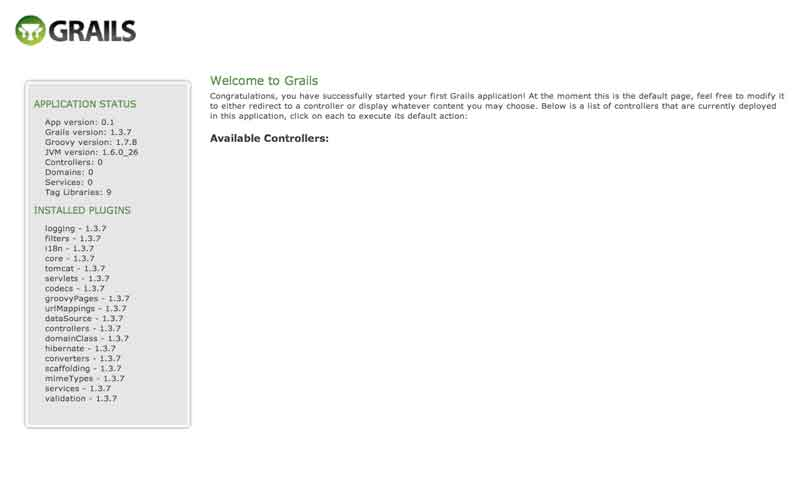
\includegraphics[width=1\textwidth]{images/firstRun.jpg}
    \caption{Primeira execução da aplicação Agenda}
    \label{fig:firstRun}
    \end{figure}
    
    O script de criação da aplicação criou a estrutura de diretórios que pode ser
    visualizada na imagem \ref{fig:appStructure}.
    
    \begin{description}
       \item [grails-app:] Diretório principal da aplicação é composto pelos diretórios a seguir:
            \begin{description}
                \item[conf:] contém os arquivos de configuração da aplicação
                \item[controllers:] contém todas as classes que executam a função de controllers na aplicação, corresponde ao C do MVC
                \item[domain:] contém as domain classes, representam entidades da aplicação, são automaticamente persistentes, corresponde ao M do MVC
                \item[i18n:] contém os arquivos properties utilizados na internacionalização
                \item[services:] contém as classes de services, são beans do Spring
                \item[taglib:] contém os arquivos de taglib customizadas para utilização nas views escritas com Groovy Server Pages (GSP)
                \item[utils:] contém utilitários específicos do Grails
                \item[views:] contém todos os arquivos GSP da aplicação, corresponde ao V do MVC
            \end{description}
        \item[lib:] Contém todos os arquivos .jar externos que são necessários a aplicação como por exemplos drivers JDBC 
        \item[scripts:] Contém scripts customizados para utilização na aplicação
        \item[src:] Contém diretórios groovy e java com código fonte que estarão disponíveis para aplicação em tempo de execução
        \item[target:] Contém todos os arquivos binários da aplicação
        \item[test:] Contém diretórios para testes de unidade e de integração
   \end{description}
    
    \begin{figure}[h!]
    \centering
    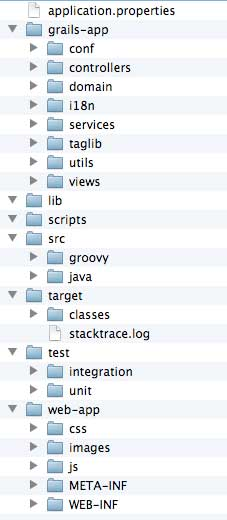
\includegraphics[width=.4\textwidth]{images/appStructure.jpg}
    \caption{Estrutura de pastas e arquivos criadas}
    \label{fig:appStructure}
    \end{figure}

\subsubsection{Criando Domain Classes - Os Contatos da Aplicação}

    Segundo \cite{pragmaticGrails:2009} o coração do grails está nas Domain Classes.
    Elas são classes que representam o domínio do negócio, seus relacionamentos e
    são persistentes. Existe a convenção que uma Domain Class está diretamente 
    ligada a uma tabela em um banco de dados.
    
    Agora que já se sabe o que é uma Domain Class, é possível criar a primeira
    classe do sistema de contatos. A classe Contato, que representa um contato.
    Um contato no sistema possui os seguintes atributos:
    
    \begin{description}
        \item[nome:] Representa o nome do contato;
        \item[email:] Representa o email do contato;
    \end{description}
    
    Para a criar uma classe de domínio utiliza-se o comando: 

    \begin{lstlisting}[language=]
       grails create-domain-class <[pacote.]NomeDaClasse>
    \end{lstlisting}
    
    onde:
    
    \begin{description}
        \item[pacote:] é opcional e representa o nome do pacote que a classe 
                      pertencerá, caso não informado, tem por valor padrão o nome
                      da aplicação;
        \item[NomeDaClasse:] é obrigatório e representa o nome da classe que será
                             criada.
    \end{description}
    
    Assim, para criar a classe Contato devemos executar o comando:
    
    \begin{lstlisting}[language=]
        grails create-domain-class agenda.Contato
    \end{lstlisting}
    
    Com isto o framework cria uma classe chamada Contato dentro do pacote agenda 
    e um teste unitário chamado ContatoTest também dentro do pacote agenda.
    
    O resultado final incluindo as propriedades inseridas manualmente pode ser visto
    nas listagens \ref{ContactV1} e \ref{ContactTestV1} a seguir.
    
    \lstinputlisting[
                      style=Groovy,
                      caption=Domain Class Contact com propriedades name e email,
                      label=ContactV1
                    ]
                    {src/groovy/agenda/contato/ContatoV1.groovy}

   \lstinputlisting[
                      style=Groovy,
                      caption=Teste Unitário da classe Contato.groovy,
                      label=ContactTestV1
                    ]
                    {src/groovy/agenda/contato/ContatoTestsV1.groovy}

    Além das propriedades que foram inseridas, o framework insere automaticamente
    na domain class duas propriedades: \textbf{id} e \textbf{version} e vários métodos.
    É possível por exemplo, com o pouco código existente, salvar, atualizar, ler
    e excluir do banco de dados. Tudo isso é possível pela natureza do Groovy, 
    os métodos são dinâmicamente criados e injetados na classe.

\subsubsection{Acessando a aplicação}

    Até o presente momento foi criada uma Domain Class e seus respectivos testes.
    Para adicionar alguma lógica ao projeto, é preciso criar um \emph{Controller}.
    Os controllers são responsáveis pela ligação entre as Domain Classes e as Views.
    Assim como para todos os recursos necessários criados até agora existe um comando
    para a facilitar a automatização, para criar um controller é necessário utilizar
    o seguinte comando:
    
    \begin{lstlisting}[language=]
          grails create-controller Contato
    \end{lstlisting}
    
    A execução do comando resultará na criação da classe ContatoController dentro
    da pasta de controllers (grails-app/controllers), o seu conteúdo é exibido na
    listagem \ref{ContactControllerV1}.
    
    \lstinputlisting[
                     style=Groovy,
                     caption=ContatoController gerado pelo comando create-controller,
                     label=ContactControllerV1
                   ]
                   {src/groovy/agenda/contato/ContatoControllerV1.groovy}
                   
    O controller criado possui apenas um método chamado index. Os métodos em um 
    controller são chamados de actions. Até o presente momento, este controller
    não executa nenhuma ação. Entretanto é possível, com poucas modificações, criar
    funcionalidades básicas de um CRUD (Create, Retrieve, Update e Delete) sobre 
    a Domain Class Contato. A listagem \ref{ContactControllerV2} demostra uma outra
    funcionalidade do framework, \emph{dynamic scaffolding}. 
    
    \lstinputlisting[
                     style=Groovy,
                     caption=ContatoController com scaffolding,
                     label=ContactControllerV2
                   ]
                   {src/groovy/agenda/contato/ContatoControllerV2.groovy}

    
    Ao executar a aplicação o resultado é o que pode ser visto na imagem \ref{fig:contactScaffold1}.

    \begin{figure}[h!]
       \centering
       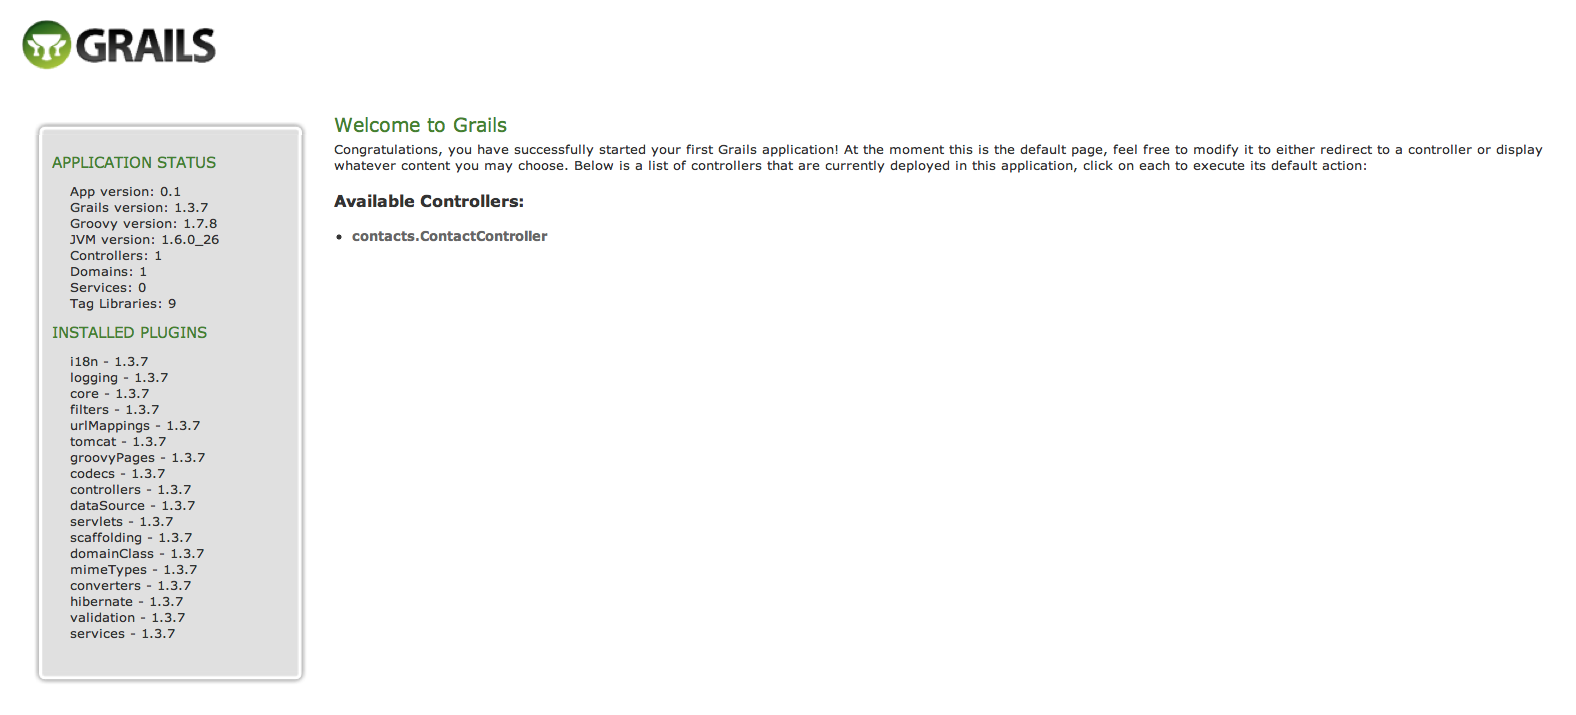
\includegraphics[width=1\textwidth]{images/contactControllerScaffold.png}
       \caption{Controller de Contatos}
       \label{fig:contactScaffold1}
   \end{figure}
   
   Ao clicar em agenda.ContatoController a aplicação redireciona o usuário para
   a página gerada pelo scaffold, como pode-se ver na figura \ref{fig:contactScaffold2}.
   
   \begin{figure}[h!]
      \centering
      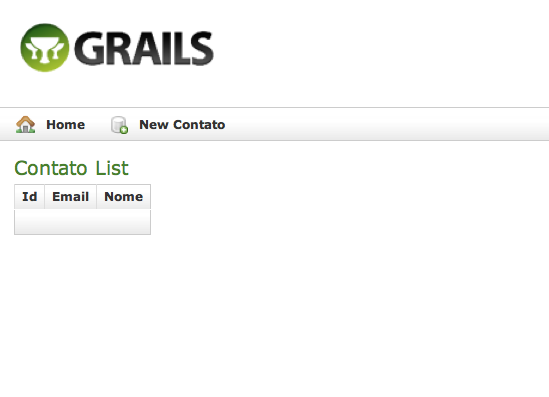
\includegraphics[width=.4\textwidth]{images/contactControllerScaffold2.png}
      \caption{Scaffolding de Contatos}
      \label{fig:contactScaffold2}
  \end{figure}
  
  Nessa página é possível disparar a criação de novos contatos e ver uma listagem
  dos contatos existentes. Como nesse momento não existe nenhum cadastrado a listagem
  não apresenta nenhum valor. A figura \ref{fig:createContactScaffold} mostra a 
  página gerada dinamicamente pelo scaffold que permite a criação de novos \textbf{contatos}.
  
   \begin{figure}[h!]
      \centering
      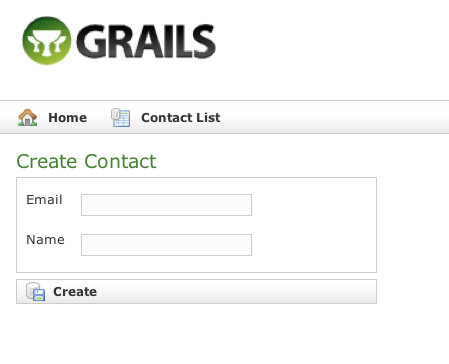
\includegraphics[width=.4\textwidth]{images/createContactScaffold.png}
      \caption{Página de criação de novos contatos gerada dinamicamente pelo scaffold}
      \label{fig:createContactScaffold}
  \end{figure}
  
  Após a criação do registro é exibida a página de exibição de contatos como pode 
  ser observado na figura \ref{fig:showContactScaffold} e na página de listagem
  agora o registro recém criado já pode ser visto, como na figura \ref{fig:listContactScaffold}.

   \begin{figure}[h!]
      \centering
      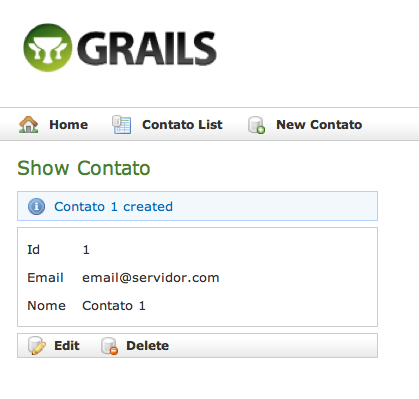
\includegraphics[width=.4\textwidth]{images/showContactScaffold.png}
      \caption{Página de exibição de um Contact gerada dinamicamente pelo scaffold}
      \label{fig:showContactScaffold}
  \end{figure}
  
   \begin{figure}[h!]
      \centering
      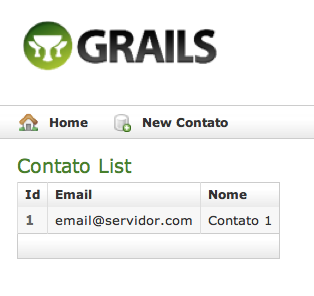
\includegraphics[width=.4\textwidth]{images/listContactScaffold.png}
      \caption{Página de exibição dos Contacts cadastrados gerada dinamicamente pelo scaffold}
      \label{fig:listContactScaffold}
  \end{figure}
  
\subsubsection{Complementando o modelo da aplicação}

  Para complementar as funcionalidades necessárias da aplicação será necessário 
  criar novas domain classes e gerar os respectivos controllers. Assim, vamos criar 
  as Domain Classes Grupo e PropriedadeContato. A Domain Class Grupo representa o
  que o nome já deixa claro. Enquanto à Domain Class PropriedadeContato representa
  o conceito de propriedades dinâmicas para o nosso Contato. Assim, é possível
  criar diversos tipos de propriedades para cada contato, e além disso, é possível
  que contatos distintos tenham propriedades distintas além do nome e email. A 
  listagem \ref{GrupoV1} mostra a Domain Class Grupo e a listagem \ref{GrupoControllerV1}
  o seu respectivo Controller. 
  
  
  \lstinputlisting[
                    style=Groovy,
                    caption=Domain Class Grupo com propriedades name,
                    label=GrupoV1
                  ]
                  {src/groovy/agenda/grupo/GrupoV1.groovy}
 
  \lstinputlisting[
                    style=Groovy,
                    caption=Controller de Grupos,
                    label=GrupoControllerV1
                  ]
                  {src/groovy/agenda/grupo/GrupoControllerV1.groovy}
 
  A listagem \ref{GrupoV1} exibe uma novidade em uma Domain Class, requisitos de 
  validação estão inseridos na classe através da closure estatica \textbf{constraints}.
  Nela estão definidas duas validações para a propriedade \textbf{nome}. A primeira
  validação diz que nome não pode ser vazio. A segunda diz que nome não pode ser
  nulo. Estas restrições serão analisadas sempre que o método \emph{validate()} 
  for invocado. Isto ocorre, por exemplo, sempre que o método \emph{save} for 
  invocado. A figura \ref{fig:ValidacaoGrupo} mostra o resultado da validação da 
  tentativa de criação de um grupo sem nome.
  
  \begin{figure}[h!]
       \centering
       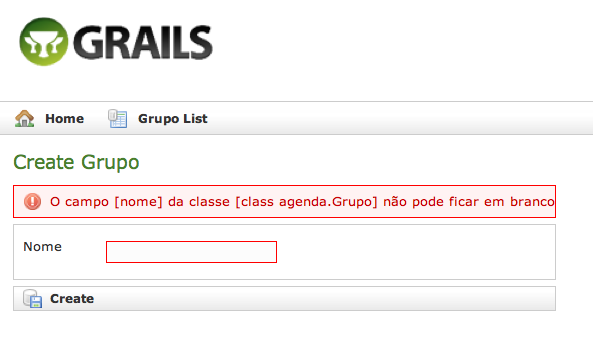
\includegraphics[width=.4\textwidth]{images/validacaoGrupo.png}
       \caption{Tentativa de criação de um grupo sem nome}
       \label{fig:ValidacaoGrupo}
   \end{figure} 
  
  Segundo \cite{pragmaticGrails:2009} existem as seguintes validações nativas no
  framework:
  
  \begin{description}
      \item[blank:(true|false)] Permite que um valor seja uma string vazia
      \item[nullable:(true|false)] Permite valores nulos
      \item[max:] Valor máximo
      \item[min:] Valor mínimo
      \item[size:] Recebe um objeto do tipo Range para determinar os extremos
      \item[maxSize:] O tamanho máximo de uma String ou Collection
      \item[minSize:] O tamanho mínimo de uma String ou Collection
      \item[inList:] Lista de valores válidos
      \item[matches:] O valor deve ser reconhecido por uma expressão regular
      \item[unique:(true|false)] Reforça a unicidade do valor no Banco de Dados
      \item[url:(true|false)] O valor deve ser uma URL válida
      \item[email:(true|false)] O valor deve ser um email válido
      \item[creditCard:(true|false)] O valor deve ser um número válido de cartão
                                     de crédito
      \item[validator:] Recebe uma closure com dois parâmetros, o primeiro sendo 
                        o valor e o segundo (opcional) a instância sendo validada
  \end{description}
  
  Além de efetuar validação a closure constraint serve para orientar o scaffolding.
  Customizações básicas podem ser criadas apenas alterando essa closure. As listagens
  \ref{PropriedadeContatoV1} e \ref{ContatoV2} exibem respectivamente as classes
  PropriedadeContato e a classe Contato atualizada com as validações.
  
  \lstinputlisting[
                      style=Groovy,
                      caption=Domain Class PropriedadeContato,
                      label=PropriedadeContatoV1
                    ]
                    {src/groovy/agenda/propriedades/PropriedadeContatoV1.groovy}
                    
  \lstinputlisting[
                    style=Groovy,
                    caption=Domain Class Contato atualizada com validações,
                    label=ContatoV2
                  ]
                  {src/groovy/agenda/contato/ContatoV2.groovy}
    
\subsubsection{Relacionamentos entre classes}
    
    Seguindo o fluxo de desenvolvimento da aplicação iremos agora tratar dos relacionamentos
    entre as classes criadas até o momento. Para a agenda, é claro que 1 Grupo
    possui várias referências à Contatos e que cada Contato pode ter várias propriedades
    além de nome e email. Para criar relacionamentos entre as classes o framework 
    apresenta o GORM. Uma abstração acima do Hibernate e que pode ser facilmente
    configurado.
    
    Propriedades Simples podem ser configuradas apenas utilizando o mecanismo de
    validação em conjunto com a definição do tipo. Esta é a razão pela qual as 
    propriedades das Domain Classes criadas até o momento utilizam tipos em vez 
    da palavra chave \textbf{def}, o que seria perfeitamente possível.
    
    Relacionamentos \textbf{1 para muitos} como no caso entre Grupo e Contato são
    configurados utilizando uma propriedade estática chamada hasMany. As chaves
    do mapa representam o nome das propriedades na classe que detém o relacionamento
    e os valores são os tipos dos objetos do relacionamento. A listagem \ref{GrupoV2}
    mostra o relacionamento entre um Grupo e seus diversos Contatos.
    
    \lstinputlisting[
                      style=Groovy,
                      caption=Relacionamento entre Grupo e os seus Contatos
                      label=GrupoV2
                    ]
                    {src/groovy/agenda/grupo/GrupoV2.groovy}
    
    A closure hasMany recebe um mapa contendo o nome das propriedades e seus respectivos
    tipos. A leitura fluída permite quase que uma tradução direta de que um Grupo
    possui muitos Contatos.
    
    
    

%iniciar uma subseção e falar sobre o grails
%incluir:
%   introdução ao grails -> DONE
%   instalação -> DONE
%   descrição da aplicação (Google Contacts Clone) -> DONE
%   script de criação da aplicação -> DONE
%   convention-over-configuration -> DONE
%   domain classes -> DONE
%   controllers -> DONE
%   scaffolding -> DONE
%   validação -> DONE
%   GORM
%   views
%       GSP
%   plugins
%\section{Figures and Captions}\label{sec:figs}
%
%Figure and table captions should be centered if less than one line
%(Figure~\ref{fig:exampleFig1}), otherwise justified and indented by 0.8cm on
%both margins, as shown in Figure~\ref{fig:exampleFig2}. The caption font must
%be Helvetica, 10 point, boldface, with 6 points of space before and after each
%caption.
%
%\begin{figure}[ht]
%\centering
%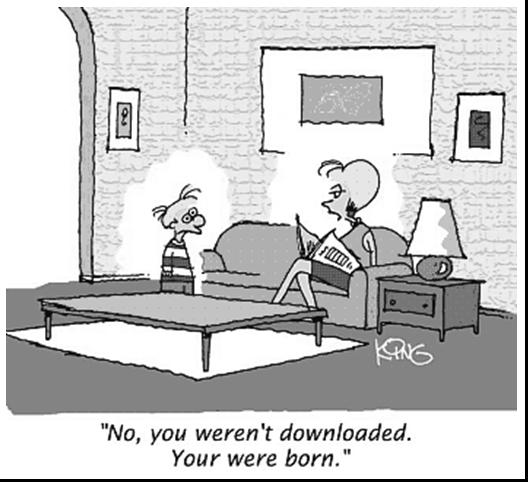
\includegraphics[width=.5\textwidth]{fig1.jpg}
%\caption{A typical figure}
%\label{fig:exampleFig1}
%\end{figure}
%
%\begin{figure}[ht]
%\centering
%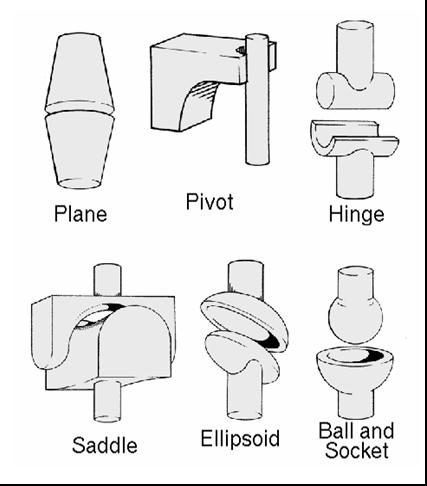
\includegraphics[width=.3\textwidth]{fig2.jpg}
%\caption{This figure is an example of a figure caption taking more than one
%  line and justified considering margins mentioned in Section~\ref{sec:figs}.}
%\label{fig:exampleFig2}
%\end{figure}
%
%In tables, try to avoid the use of colored or shaded backgrounds, and avoid
%thick, doubled, or unnecessary framing lines. When reporting empirical data,
%do not use more decimal digits than warranted by their precision and
%reproducibility. Table caption must be placed before the table (see Table 1)
%and the font used must also be Helvetica, 10 point, boldface, with 6 points of
%space before and after each caption.
%
%\begin{table}[ht]
%\centering
%\caption{Variables to be considered on the evaluation of interaction
%  techniques}
%\label{tab:exTable1}
%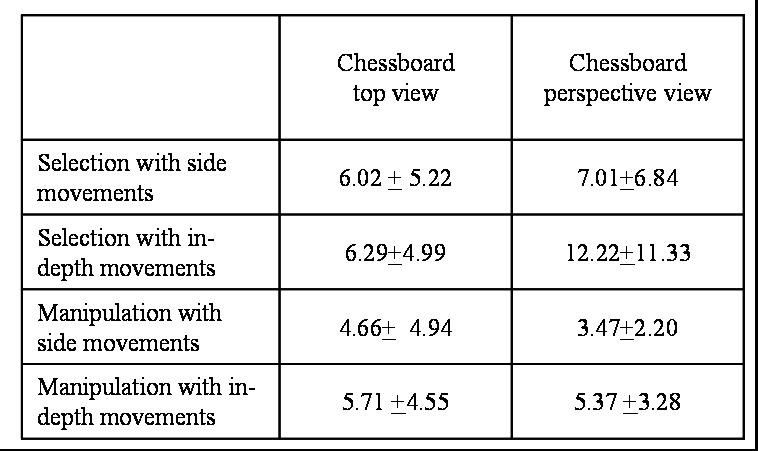
\includegraphics[width=.7\textwidth]{table.jpg}
%\end{table}
%
%\section{Images}
%
%All images and illustrations should be in black-and-white, or gray tones,
%excepting for the papers that will be electronically available (on CD-ROMs,
%internet, etc.). The image resolution on paper should be about 600 dpi for
%black-and-white images, and 150-300 dpi for grayscale images.  Do not include
%images with excessive resolution, as they may take hours to print, without any
%visible difference in the result. 
%
%
%Bibliographic references must be unambiguous and uniform.  We recommend giving
%the author names references in brackets, e.g. \cite{knuth:84},
%\cite{boulic:91}, and \cite{smith:99} and \cite{beginingGroovy:2008}, \cite{groovy}, \cite{groovy:refcard}.
%
%The references must be listed using 12 point font size, with 6 points of space
%before each reference. The first line of each reference should not be
%indented, while the subsequent should be indented by 0.5 cm.

\bibliographystyle{sbc}
\bibliography{artigo}

\end{document}
